% Maximal gaps g after p (record holders up to 10^9, 30 of them, blue; the record below 4e18, g = 1476 after 1425172824437699411, red) against u = log^2 p; dashed: g = log^2 p. Largest computed here: g = 282 after 436273009.
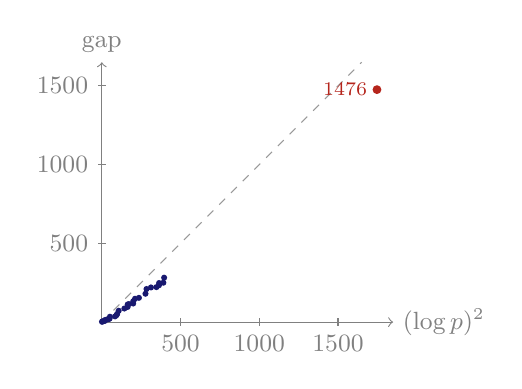
\begin{tikzpicture}[font=\small]
\draw[black!50,->] (0,0) -- (3.700,0) node[right] {$(\log p)^2$};
\draw[black!50,->] (0,0) -- (0,3.300) node[above] {gap};
\draw[black!40,dashed] (0,0) -- (3.300,3.300);
\draw[black!50] (1.000,0.05) -- (1.000,-0.05) node[below] {$500$};
\draw[black!50] (0.05,1.000) -- (-0.05,1.000) node[left] {$500$};
\draw[black!50] (2.000,0.05) -- (2.000,-0.05) node[below] {$1000$};
\draw[black!50] (0.05,2.000) -- (-0.05,2.000) node[left] {$1000$};
\draw[black!50] (3.000,0.05) -- (3.000,-0.05) node[below] {$1500$};
\draw[black!50] (0.05,3.000) -- (-0.05,3.000) node[left] {$1500$};
\fill[MidnightBlue] (0.0024,0.0040) circle (1.1pt);
\fill[MidnightBlue] (0.0076,0.0080) circle (1.1pt);
\fill[MidnightBlue] (0.0197,0.0120) circle (1.1pt);
\fill[MidnightBlue] (0.0403,0.0160) circle (1.1pt);
\fill[MidnightBlue] (0.0447,0.0280) circle (1.1pt);
\fill[MidnightBlue] (0.0784,0.0360) circle (1.1pt);
\fill[MidnightBlue] (0.0921,0.0400) circle (1.1pt);
\fill[MidnightBlue] (0.0988,0.0440) circle (1.1pt);
\fill[MidnightBlue] (0.1034,0.0680) circle (1.1pt);
\fill[MidnightBlue] (0.1680,0.0720) circle (1.1pt);
\fill[MidnightBlue] (0.1866,0.0880) circle (1.1pt);
\fill[MidnightBlue] (0.1954,0.1040) circle (1.1pt);
\fill[MidnightBlue] (0.2144,0.1440) circle (1.1pt);
\fill[MidnightBlue] (0.2859,0.1720) circle (1.1pt);
\fill[MidnightBlue] (0.3275,0.1920) circle (1.1pt);
\fill[MidnightBlue] (0.3288,0.2240) circle (1.1pt);
\fill[MidnightBlue] (0.3436,0.2280) circle (1.1pt);
\fill[MidnightBlue] (0.3985,0.2360) circle (1.1pt);
\fill[MidnightBlue] (0.3988,0.2640) circle (1.1pt);
\fill[MidnightBlue] (0.4213,0.2960) circle (1.1pt);
\fill[MidnightBlue] (0.4714,0.3080) circle (1.1pt);
\fill[MidnightBlue] (0.5546,0.3600) circle (1.1pt);
\fill[MidnightBlue] (0.5680,0.4200) circle (1.1pt);
\fill[MidnightBlue] (0.6246,0.4400) circle (1.1pt);
\fill[MidnightBlue] (0.6935,0.4440) circle (1.1pt);
\fill[MidnightBlue] (0.7266,0.4680) circle (1.1pt);
\fill[MidnightBlue] (0.7275,0.4960) circle (1.1pt);
\fill[MidnightBlue] (0.7820,0.5000) circle (1.1pt);
\fill[MidnightBlue] (0.7915,0.5640) circle (1.1pt);
\fill[BrickRed] (3.4946,2.9520) circle (1.6pt) node[left,font=\scriptsize] {$1476$};
\end{tikzpicture}
